\documentclass{article}

\usepackage{fancyhdr}
\cfoot{
\vspace{1mm}\hspace{3cm}

\includegraphics[width=0.2\textwidth]{CC-BY-NC-SA.pdf}}

\renewcommand{\headrulewidth}{0pt}
\renewcommand{\footrulewidth}{0pt}
\setlength\headheight{80.0pt}
\addtolength{\textheight}{-80.0pt}

\usepackage[margin = 3cm, footskip = 30pt]{geometry}
\usepackage{amsmath}
\usepackage{blkarray}
\usepackage[table]{xcolor}
\usepackage{amssymb}
\usepackage{amsfonts}
\usepackage{enumerate}
\newcommand\bg{\cellcolor{gray!70}}

\usepackage{stackengine,graphicx}
\def\stacktype{L}
\def\useanchorwidth{T}
\newcommand\strike[1]{\stackon[3.3pt]{#1}{\rule{4.5ex}{1pt}}}
\newcommand\vstrike[1]{\stackon[0pt]{#1}{\smash{\rule[-3pt]{1pt}{2.9ex}}}}

\usepackage{tikz}
\usetikzlibrary{shapes.geometric, arrows,positioning,automata}


\makeatletter
\renewcommand*\env@matrix[1][*\c@MaxMatrixCols c]{
  \hskip -\arraycolsep
  \let\@ifnextchar\new@ifnextchar
  \array{#1}}
\makeatother

\title{Linear Algebra (Part 006)\\Linear Independence}
\author{Dr Kapil\\kapil $@$ nitkkr $\cdot$ ac $\cdot$ in\\ Department of Computer Applications\\ NIT Kurukshetra}
\date{\today}

\begin{document}
\maketitle
\thispagestyle{fancy}
\textbf{Definition}  (Linear Combination)\\
Consider a vector space $V$ and a finite number of vectors \(\vec{x}_1, \cdots \vec{x}_k \in V \). Then, every \(\vec{v} \in V\) of the form \(\vec{v} = \lambda_1\vec{x}_1 + \lambda_2\vec{x}_2 + \ldots + \lambda_k\vec{x}_k = \sum_{i=1}^{k}\lambda_i\vec{x}_i\) with $\lambda_1, \lambda_2, \cdots \lambda_k \in \mathbb{R}$ is a \textit{linear combination} of the vectors $\vec{x}_1, \cdots, \vec{x}_k$.\\

Any linear combination of vectors from a particular vector space will always be an element of the same vector space i.e.\( (\forall~c,d \in \mathbb{R}) (\vec{x_1},\vec{x_2} \in V \implies c\vec{x_1}+d\vec{x_2} \in V)\). In other words, you can say that for some arbitrary value of \((c,d \in \mathbb{R}) (\vec{x_1},\vec{x_2} \in V)\)

\begin{align}
    c \vec{x_1} \in V ~~~ (\because\text{Scalar multiplication is closed in }V) \nonumber\\
    d \vec{x_2} \in V ~~~ (\because\text{Scalar multiplication is closed in }V) \nonumber
\end{align}

\[
\because c \vec{x_1} \in V, d \vec{x_2} \in V \implies c \vec{x_1} + d \vec{x_2} \in V ~~~ (\because\text{Vector addition is closed in }V)
\]
$\vec{0} \in V$ can always be written as linear combination of $k$-vectors \begin{math}\vec{x_1}, \vec{x_2}, \cdots, \vec{x_k}\end{math} because we can keep all scalar values to be zero i.e $\vec{0} = 0\vec{x_1} + 0\vec{x_2} + \cdots + 0\vec{x_n}$

\section{Linear Independence}

Consider a vector space $V$ with $k \in \mathbb{N}$ and $\vec{x_1}, \vec{x_2}, \cdots, \vec{x_k} \in V$. If at-least one of the vectors can be represented as linear combination of other vectors then the set of vectors $\{\vec{x_1}, \vec{x_2}, \cdots, \vec{x_k}\}$ is said to be \textit{linearly dependent}.\\

The definition is equivalent to this one -- \\
A set of vectors $\mathbb{U} = {\vec{x_1}, \vec{x_2}, \cdots, \vec{x_k}}$ is said to be \textit{linearly dependent} if $\exists~\lambda_1, \cdots, \lambda_k \in \mathbb{R}$ such that $\exists \lambda_i \neq 0$ for some $1 \leq i \leq k$ and $\lambda_1\vec{x_1} + \lambda_2\vec{x_2} + \cdots + \lambda_k\vec{x_k} = \vec{0}$. i.e. at least one $\lambda_i$ is not zero and still the linear combination of vectors from $\mathbb{U}$ can generate $\vec{0}$. Then the set of vectors i.e. $\mathbb{U}$ is called linearly dependent.

But, if the negation of the above statement is true, then the set of vectors is called as \textit{linearly independent}. In other words, for set of vectors $\mathbb{U} = \{\vec{x_1}, \cdots, \vec{x_k}\}$ is said to be linear independent if none of the  vectors in the set can be expressed as linear combination of other vectors of the set, i.e. \(\nexists j \in\{1, \cdots, k\}\)  such that
    \begin{equation} \label{aa}
        x_j = \lambda_1\vec{x}_1 + \cdots + \lambda_{j-1}\vec{x}_{j-1} + \lambda_{j+1}\vec{x}_{j+1} + \cdots + \lambda_k\vec{x_k}
    \end{equation}
    does not have any solution. Bingo! we learned something new that $A\vec{x} =\vec{b}$ is not solvable, if $\vec{b}$ is linearly independent of column vectors of $A$.
    
\subsection{Proof of equivalence of two definition}
Multiplying the equation \eqref{aa} above by some non zero scalar value ($\alpha\neq 0$) and then replacing it with new scalars ($\alpha_i=\alpha\lambda_i \forall i\neq j\text{ and } \alpha_j = -\alpha$) and taking $\vec{x_j}$ term in right side, we get
\[
    \alpha_1\vec{x_1} + \alpha_2\vec{x_2} + \cdots + \alpha_j\vec{x_j} + \cdots + \alpha_k\vec{x_k} = 0.
\]
That is above equation does not have any solution if at least one of the scalar (i.e. $\alpha_j = -\alpha \neq 0$).\\
For example-
\begin{enumerate}
    \item \(\left\{\begin{pmatrix} 1 \\ 2 \end{pmatrix}, \begin{pmatrix} 4 \\ 8 \end{pmatrix}\right\}\) ~~~  is linear dependent as $\begin{pmatrix} 4 \\ 8 \end{pmatrix} = 4 \begin{pmatrix} 1 \\ 2 \end{pmatrix}$
    \item \(\left\{ \begin{pmatrix} 1 \\ 2 \end{pmatrix}, \begin{pmatrix} 3 \\ 4 \end{pmatrix}\right\}\)
   ~~~ for it to be linearly dependent $\lambda_1 + 3\lambda_2 = 0,~~2\lambda_1 + 4\lambda_2 = 0 $ should have at least one non zero solution or non-trivial solution.
\end{enumerate}
A homogeneous system of linear equations always has \textit{trivial solution} (i.e. $\vec{0}$) but, in some cases it can also have non-zero solutions known as \textit{non-trivial solutions}.\\
So, linear dependence is equivalent to asking for infinite solutions for homogeneous system of linear equations. And you know that determinant associated with above system is not zero and hence it has unique solution that is $\lambda_1 = \lambda_2 = 0$. So they should be linearly independent. Now, you can try few more examples to know if the set of vectors is linear dependent or linearly independent-
\begin{enumerate}
    \item \(\left\{ \begin{pmatrix} 1 \\ 0 \end{pmatrix}, \begin{pmatrix} 0 \\ 1 \end{pmatrix}, \begin{pmatrix} 2 \\ 3 \end{pmatrix}\right\}\)
    \item \(\left\{\begin{pmatrix} 2 \\ 2 \end{pmatrix}, \begin{pmatrix} -2 \\ 2 \end{pmatrix}\right\}\)
    \item \(\left\{ \begin{pmatrix} 2 \\ 3 \end{pmatrix}, \begin{pmatrix} 4 \\ 7 \end{pmatrix}, \begin{pmatrix} 3 \\ 2 \end{pmatrix} \right\}\).
\end{enumerate}

We can also think about linearly dependence of set of vectors with the help of matrices. Consider a matrix $A$, keeping all the vectors of the set in question in its column. If some non-zero linear combination of column vectors of $A$ generates $\vec{0}$ (i.e. $A\vec{x}=\vec{0}$), then the set is linearly dependent. \\

Further, if you think about Gauss elimination in each step, a row is replaced by linear combination of the rows of the matrix. Here, we also ensure that the multiplier of replaced row should not be zero. Therefore, when moving from one system of linear equations to another but equivalent system of linear equations with Gauss elimination, if we get a row entirely zero, then it means that the row vectors of the matrix are linearly dependent.\\

Geometrically, in a set of two vectors, the set is linearly dependent if both the vectors have same direction (magnitude may be different). And the area of the parallelogram made of up two vectors is the quantity determined by determinants. Therefore, we have a straight forward technique to find if the two vectors are linearly dependent or independent. The determinant will be zero or non-zero in respective cases.

\textbf{Exercise}
\begin{tikzpicture}
\fill[gray!50!white] (0,0) -- (4,1) -- (6,6) -- (2,5);
\draw[->,thick] (0,0) -- (7,0);
\draw[->,thick] (0,0) -- (0,7);
\draw[->,thick] (0,0) -- (4,1) node[pos=1.2]{$(a,b)$};
\draw[->,thick] (4,1) -- (6,6) node[pos=1.1] {$(a+c,b+d)$};
\draw [->,thick] (0,0) -- (2,5) node[above]{$(c,d)$};
\draw [->,thick](2,5) -- (6,6);
\draw [dashed] (6,0) -- (4,1) -- (0,1) node[left]{$(0,b)$} ;
\draw [dashed] (6,6) -- (6,0) node[below] {$(a+c,0)$};
\node at (3,3) {$ad-bc$};
\end{tikzpicture}\\
Prove that the area of parallelogram shaded here is same as that of determinants of \(\begin{vmatrix} a & c \\ b & d \end{vmatrix}\).\\

Some important points to notice about linear independence.
\begin{enumerate}
    \item A set of vectors will always be either linearly dependent or linear independent (no third option).
    \item If at least one vector is zero, then the set is linear dependent.
    \item If at least one vector is duplicate of some other vector in the set, then also the set is linear dependent
    \item A practical way of checking if vectors ~~$\vec{v}_1, \vec{v}_2, \vec{v}_3, \dots, \vec{v}_k \in V$ are linear dependent is to construct a  matrix, $B$ whose row vectors are vectors of the set. Apply Gaussian elimination to achieve row-echelon form. If a completely zero row appears, then set is linearly dependent.
    \item Another way is to construct a matrix, $A$ whose column vectors are the vectors of the set. Now, solve $A\vec{x}=\vec{0}$ and check if you have at least one non-zero solution for the set of vectors to be linearly dependent.
\end{enumerate}
Moreover, you can note that-
\begin{itemize}
    \item Pivot columns of $A$ and pivot rows of $B$ indicate the linearly independent vectors.
    \item Non-pivot column vectors of $A$ and non-pivot rows of $B$ are linearly dependent on the pivot columns of the left of the column of $A$ or above the row vector of $B$.
\end{itemize}
So, all the columns of $A$ are linear independent if all the columns has at least one pivot element. Similar, notion you can make for the rows of $B$.\\

\textbf{Example}
\[\left[\begin{array}{ccc}
    \bg1 & 3 & 0\\
    0 &0 &\bg2
    \end{array}\right]
\]
Here, grey items are pivot elements of reduced row echelon form. Now notice that-
\begin{enumerate}
    \item First and third column are independent column vectors.
    \item Obviously, first column is always linearly independent because there is no column on the left of it. Except only if the first vector is entirely zero. 
    \item Second column vector (even the original vector too) is linearly dependent on the first column vector (here it is three times the first column).
    \item Third column vector (the original one too, before Gauss elimination) is linearly independent of left two column vectors.
\end{enumerate}

\textbf{Questions.} Check if the following set of vectors are linearly dependent or linearly independent\\
\begin{enumerate} [i.]
    \item $ \begin{bmatrix}1\\2\\-3\\4 \end{bmatrix},~~~
        \begin{bmatrix}1\\1\\0\\2 \end{bmatrix} ,~~~
        \begin{bmatrix}-1\\-2\\1\\1\end{bmatrix} $
    \item $ \begin{bmatrix}1\\0\end{bmatrix},~~~
        \begin{bmatrix}0\\1 \end{bmatrix} $
    \item  $\begin{bmatrix}1\\0 \end{bmatrix},~~~
        \begin{bmatrix}0\\1\end{bmatrix} ,~~~
        \begin{bmatrix}a\\b\end{bmatrix} $
    \item $ \begin{bmatrix}1\\1\\1\end{bmatrix},~~~
        \begin{bmatrix}2\\1\\-2\end{bmatrix} ,~~~
        \begin{bmatrix}-3\\0\\1\end{bmatrix} ,~~~ 
        \begin{bmatrix}4\\2\\1\end{bmatrix} $ 
\end{enumerate}
Notice the relation between (iv) and (i).

Although about following section we have already talked in Part004b and previously in this Part, we are writing here again for the sake of putting the things together.

\section{Homogeneous system of linear Equations}
A system of linear equations is \textit{homogeneous} if and only if all constant terms of all the equations are zero. That is it should have $A\vec{x} = \vec{0}$ matrix equation form. A homogeneous system of linear equations must always have a trivial solution i.e. $\vec{x} = \vec{0}$. But it is possible to have some non-zero (non-trivial) solutions of $A\vec{x} = \vec{0}$. In that case it must have infinite solution. (Why?)\\

The general solution of any system of linear equations is a sum of particular solution and the solution of corresponding homogeneous system of equations. Basically, particular solution asks for unique solution when free variables are set to zero and corresponding to the constant term $\vec{b}$ of the matrix equation.\\

And the homogeneous solution corresponds to all possible solution that can create zeros instead of $\vec{b}$ by assigning parametric value to free variables. \\

 \[ \text{i.e. To solve }A\vec{x} = \vec{b}\]
\begin{enumerate} [I]
    \item $A\vec{x} = \vec{b}$ is solved only for pivot columns. The solution is denoted by $\vec{x}_p$.
    \item $A\vec{x} = \vec{0}$ is solved for (especially non-zero) solutions of homogeneous system. The solution is denoted by $\vec{x}_h$.
\end{enumerate}
And the Total/General solution is $\vec{x} = \vec{x}_p + \vec{x}_h$.
\subsection{Relationship among vectors generated from linear combinations of linearly independent vectors}
Consider a vector space $V$ with $k$ linearly independent vectors $B = \{\vec{b}_1$,\ldots,$\vec{b}_k\}$ and a set of $m$ vectors, $X =  \{\vec{x}_1$,\ldots,$\vec{x}_m\}$ generated from linear combinations of vectors in $B$. Therefore, any vector, $x_i$ from $X$ can be written as-
\[\vec{x}_j= \sum_{i=1}^{k} \lambda_{ji}\vec{b}_i~~~~\forall j\in \{1,\ldots,m\}\]
So, if\[B = \begin{bmatrix} \vstrike{$\vec{b}_1$}\dots\vstrike{$\vec{b}_k$}\end{bmatrix}\]
then,\[\vec{x}_j = B\vec{\lambda}_j~,~~~\vec{\lambda}_j = 
\begin{bmatrix}
\lambda_{1j}\\
\vdots\\
\lambda_{kj}
\end{bmatrix},~~~~
 \text{where}~~~j\in \begin{Bmatrix} 1,\dots,m\end{Bmatrix}
\]
or 
\[
X = \begin{bmatrix}
\vstrike{$\vec{x}_1$}\dots\vstrike{$\vec{x}_m$}
\end{bmatrix} = 
B\Lambda = \begin{bmatrix}
\vstrike{$\vec{b}_1$}\dots\vstrike{$\vec{b}_k$}
\end{bmatrix}
\begin{bmatrix}
\lambda_{11} & \dots & \lambda_{1m}\\
\vdots &\ddots  & \vdots\\
\lambda_{k1} & \dots& \lambda_{km}
\end{bmatrix}\text{, where }\Lambda = \begin{bmatrix} \vstrike{$\vec{\lambda}_1$}\dots\vstrike{$\vec{\lambda}_m$}\end{bmatrix}
\]
Now, if we want to know $\vec{x}_1,\dots\vec{x}_m$ are \textbf{linear independent} or \textbf{linear dependent}.

For this purpose, we should check $\sum_{j=1}^{m} \psi_j \vec{x}_j = \vec{0}$  
\[
\sum_{j=1}^{m} \psi_j \vec{x}_j = \sum_{j=1}^{m} \psi_j B \vec{\lambda}_j = \sum_{j=1}^{m} B( \psi_j \vec{\lambda}_j )
\]
$\therefore$ The equation of linear independence of $\vec{x}_j$ is directly dependent on linear dependence of $\vec{\lambda}_j$ i.e. $x_j$ are linearly independent if and only if $\vec{\lambda}_j$ are linear independent.

In particular, $m$- linear combinations of $k$ linearly independent vectors $\vec{x}_1,\dots,\vec{x}_k$ are \textit{linear dependent} if $m > K$

Check exercise 2.15 from book. (Chapter 2, Page 43)
\end{document}